\documentclass[UTF8,12pt,a4paper]{ctexart}

\usepackage{amsmath}
\usepackage{cases}
\usepackage{cite}
\usepackage{graphicx}
\usepackage{enumerate}
\usepackage{algorithm}
\usepackage{caption}   % \caption*需要
\usepackage{subcaption} % 子图布局
\usepackage[noend]{algpseudocode} %algorithmicx
\makeatletter
\renewcommand{\fnum@algorithm}{\fname@algorithm}
\makeatother
\renewcommand{\algorithmicrequire}{\textbf{Input:}}
\renewcommand{\algorithmicensure}{\textbf{Output:}}
\usepackage[margin=1in]{geometry}
\geometry{a4paper}
\usepackage{fancyhdr}
\pagestyle{fancy}
\fancyhf{}
\usepackage{xcolor}

% ------------------------- 代码展示设置 -------------------------
% ------------------- MATLAB 代码展示风格(DSP 专用) -----------------
\usepackage{listings}
\usepackage{xcolor}

% 定义 MATLAB 风格
\lstdefinestyle{matlab-dsp}{
    language=Matlab,
    basicstyle=\ttfamily\small,
    keywordstyle=\color{blue}\bfseries,
    commentstyle=\color{green!50!black}\itshape,
    stringstyle=\color{brown},
    numbers=left,
    numberstyle=\tiny\color{gray},
    stepnumber=1,
    numbersep=5pt,
    backgroundcolor=\color{white},
    showspaces=false,
    showstringspaces=false,
    showtabs=false,
    frame=single,
    rulecolor=\color{black},
    tabsize=4,
    captionpos=b,
    breaklines=true,
    breakatwhitespace=true,
    escapeinside={\%*}{*)},
    % MATLAB 关键字(基础)
    morekeywords={if, else, elseif, end, for, while, switch, case, otherwise, try, catch, function, return, break, continue, pause, clear, clc, close, disp, plot, figure, hold, grid, xlabel, ylabel, title, xlim, ylim, fft, ifft, freqz, filter, conv, zeros, ones, length, size, abs, angle, unwrap, real, imag, exp, sin, cos, pi, inf, nan, true, false, struct, cell, classdef, properties, methods},
    % DSP 常用函数(重点突出)
    morekeywords=[2]{freqz, zplane, fftshift, ifftshift, fft, ifft, filter, filtfilt, butter, cheby1, ellip, fir1, fir2, remez, sinc, rectwin, hamming, hanning, blackman, kaiser, decimate, interp, resample, xcorr, conv, corrcoef, pwelch, spectrogram, tf, zpk, ss, bode, impulse, step, lsim, unwrap, angle, abs, real, imag, db, mag2db, db2mag, rms, mean, std, var, cov, eig, svd, lpc, prony, residuez, tf2zp, zp2tf, tf2sos, sos2tf, sosfilt, upfirdn, buffer, overlapadd, fftfilt},
    % 常量/特殊变量
    morekeywords=[3]{pi, Inf, NaN, eps, i, j, nargin, nargout, varargin, varargout},
    % 注释以 % 开头
    comment=[l]{\%},
    % 字符串用单引号或双引号
    alsoletter={.}, % 允许 . 在标识符中(如 x.y)
    sensitive=true
}

% 默认使用此样式
\lstset{style=matlab-dsp}

% ------------------- 设置超链接,便于跳转 -----------------
\usepackage{enumitem}
\usepackage{hyperref}
\hypersetup{
    pdfborder={0 0 0},    % 消除超链接边框
    colorlinks=true,       % 将边框改为颜色标记(可选)
    linkcolor=black,       % 内部链接颜色(目录、引用等)
    citecolor=black,       % 引用颜色
    urlcolor=blue          % URL链接颜色(保持蓝色以便区分)
}




% ------------------------ 标题区 ----------------------------
\title{DSP 实验二报告}
\author{
	姓名:\underline{冯峻}~~~~~~
	学号:\underline{523031910148}~~~~~~}
\date{\today}
\pagenumbering{arabic}

\begin{document}



% ------------------------ 页眉和页脚 ----------------------------
\fancyhead[L]{冯峻}
\fancyhead[C]{实验二}
\fancyfoot[C]{\thepage}

\maketitle
\tableofcontents
\newpage

% ============================================================
% 实验一:3-31 有限长序列的 DTFT 幅度与相位
% ============================================================
\section{实验一:3-31 有限长序列的 DTFT 幅度与相位}

\subsection{题目内容}
画出下列序列傅里叶变换的幅度和相位。

(a) $x[n] = \{4,3,2,1,2,3,4\}$, $n = \{0,1,2,3,4,5,6\}$;

(b) $x[n] = \{4,3,2,1,0,-1,-2,-3,-4\}$, $n = \{0,1,2,3,4,5,6,7,8\}$。

注意观察幅度和相位的对称性。

(提示: 可以调用的函数有 \texttt{fplot()}、\texttt{abs()}、\texttt{angle()} 或 \texttt{freqz()}、\texttt{exp()} 等)

\subsection{实验结果}

3-31(a)的MATLAB仿真图像见图\ref{fig:3-31a}:

\begin{figure}[htbp]
    \centering
    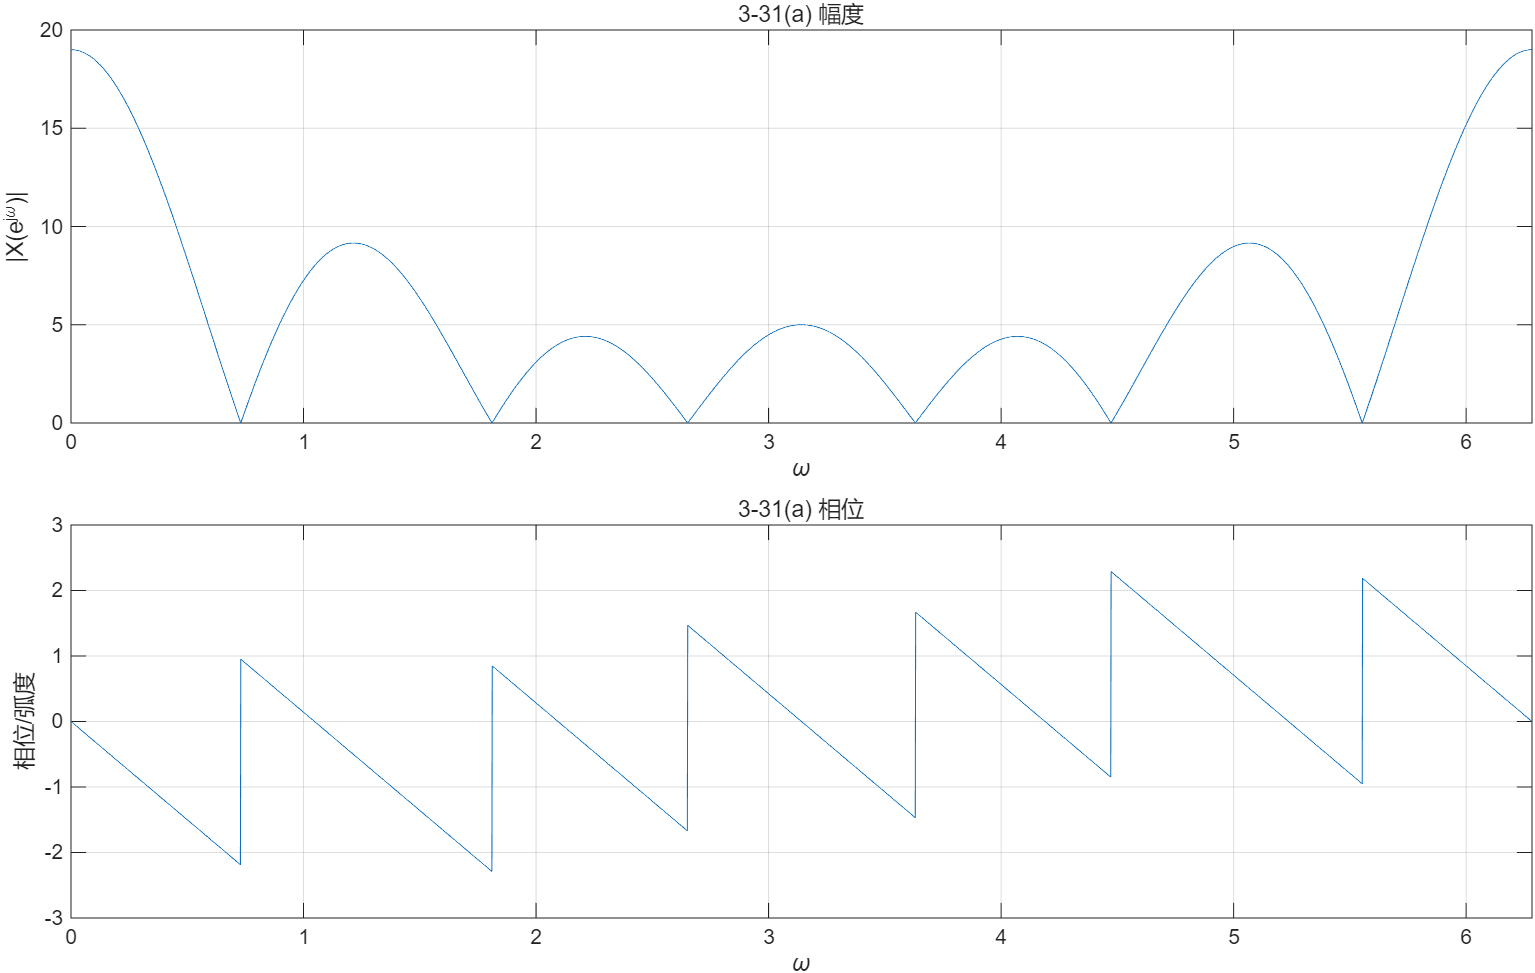
\includegraphics[width=0.8\textwidth]{3-31(a).png}
    \caption{3-31(a) DTFT幅度与相位}
    \label{fig:3-31a}
\end{figure}

3-31(b)的MATLAB仿真图像见图\ref{fig:3-31b}:

\begin{figure}[htbp]
    \centering
    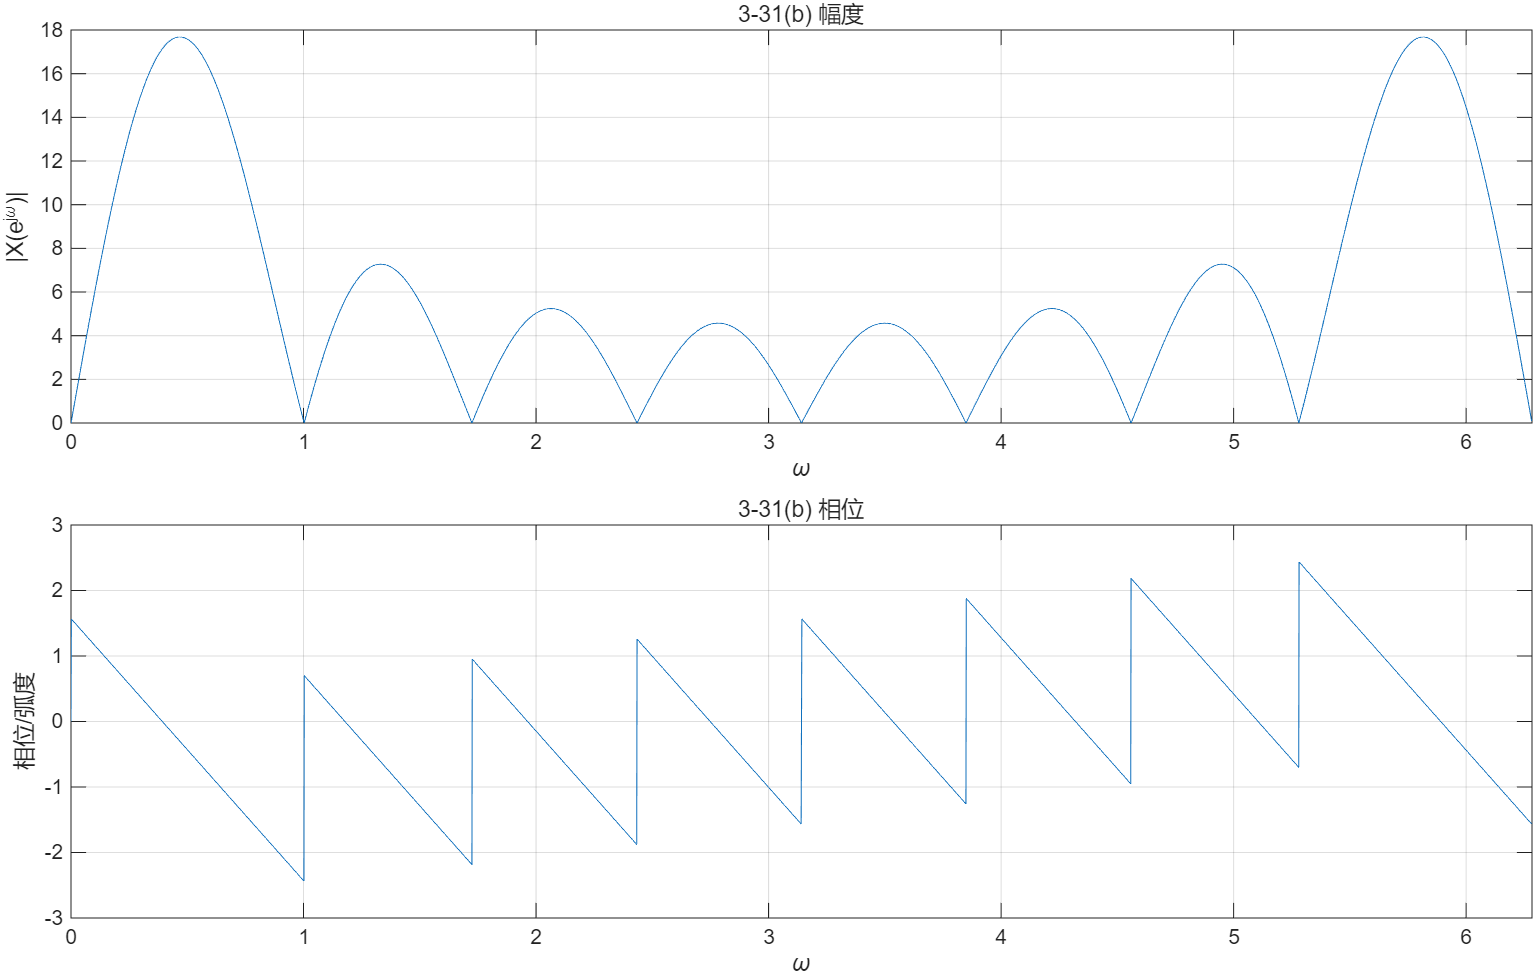
\includegraphics[width=0.8\textwidth]{3-31(b).png}
    \caption{3-31(b) DTFT幅度与相位}
    \label{fig:3-31b}
\end{figure}

\subsection{实验分析}

这两个序列都是实值序列:

\subsubsection{幅度对称性}

$y[n]=x[n+3]$是实值序列,则$Y(e^{j\omega})$满足:
$$Y(e^{j\omega})=Y(e^{-j\omega})$$
因此$$|Y(e^{j\omega})|=|Y(e^{-j\omega})|$$
因此$$|e^{j3\omega}X(e^{j\omega})|=|e^{-j3\omega}X(e^{-j\omega})|$$
因此:$$|X(e^{j\omega})|=|X(e^{-j\omega})|$$
因此$|X(e^{j\omega})|$关于$x=0(+2k\pi)$偶对称,又:
$$|X(e^{j(\pi-\omega)})|=|X(e^{j(-\pi-\omega)})|=|X(e^{j(\pi+\omega)})|$$
因此$|X(e^{j\omega})|$关于$x=\pi(+2k\pi)$偶对称

综上所述:$|X(e^{j\omega})|$关于$x=k\pi$\textbf{偶对称}

\subsubsection{相位对称性}

$Y(e^{j\omega})$满足:
$$\angle [Y(e^{j\omega})]=-\angle [Y(e^{-j\omega})]$$
即:
$$ 3\omega + \angle[X(e^{j\omega})]=-\angle[X(e^{-j\omega})]-(-3\omega)$$
即:
$$\angle [X(e^{j\omega})]=-\angle [X(e^{-j\omega})]$$
因此,与幅度对称性的分析相同,很容易发现:
$\angle[X(e^{j\omega})]$关于$x=k\pi$\textbf{奇对称}

\subsubsection{广义线性相位序列}

此外,我们发现,这两个序列分别关于$x=3$和$x=4$呈偶对称和奇对称,其代表的系统分别是I类系统和III类系统,其频率响应分别是:
$$3\text{-}31(a): X(e^{j\omega})=e^{-j\omega\frac{M}{2}}\sum_{n=0}^{M}x[n]\cos[\omega(n-\frac{M}{2})]$$
和:
$$3\text{-}31(b): X(e^{j\omega})=e^{-j\omega\frac{M}{2}+j\frac{\pi}{2}}\sum_{n=0}^{M}x[n]\cos[\omega(n-\frac{M}{2})+\frac{\pi}{2}]$$
,可以发现,则两个序列的傅里叶变换的相位响应的斜率一定是:-3和-4,与图中相同。

% ============================================================
% 实验二:3-34 周期序列的 DFS 与 DTFT
% ============================================================
\section{实验二:3-34 周期序列的 DFS 与 DTFT}

\subsection{题目内容}

画出以下周期序列的 DFS 和傅里叶变换,其中 $N$ 为周期。

(a) $\tilde{x}[n] = \cos(0.8\pi n) + \cos(0.1\pi n)$

(b) $\tilde{x}[n] = \{0,0,1,0,0\}$, $N=5$

(c) $\tilde{x}[n] = \{3,-3,3,-3\}$, $N=4$

\subsection{实验结果}

3-34(a)的MATLAB仿真图像(DFS的幅度和相位以及DTFT的幅度和相位)见图\ref{fig:3-34a}:

\begin{figure}[htbp]
    \centering
    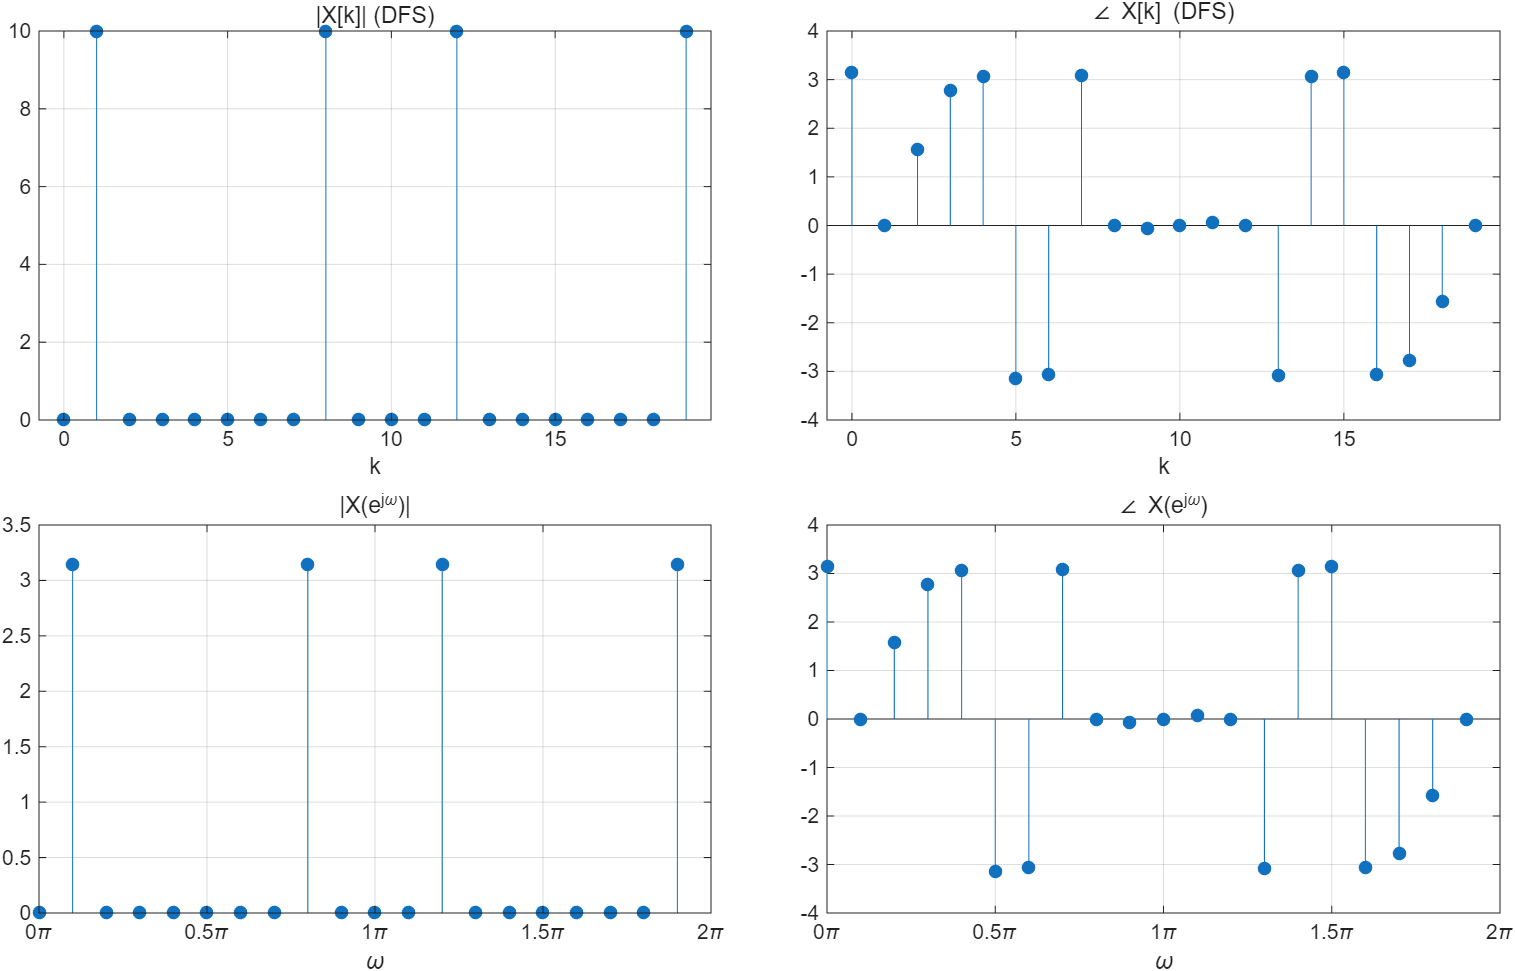
\includegraphics[width=0.8\textwidth]{3-34(a) N=20.png}
    \caption{3-34(a) N=20 DFS与DTFT}
    \label{fig:3-34a}
\end{figure}

3-34(b)的MATLAB仿真图像(DFS的幅度和相位以及DTFT的幅度和相位)见图\ref{fig:3-34b}:

\begin{figure}[htbp]
    \centering
    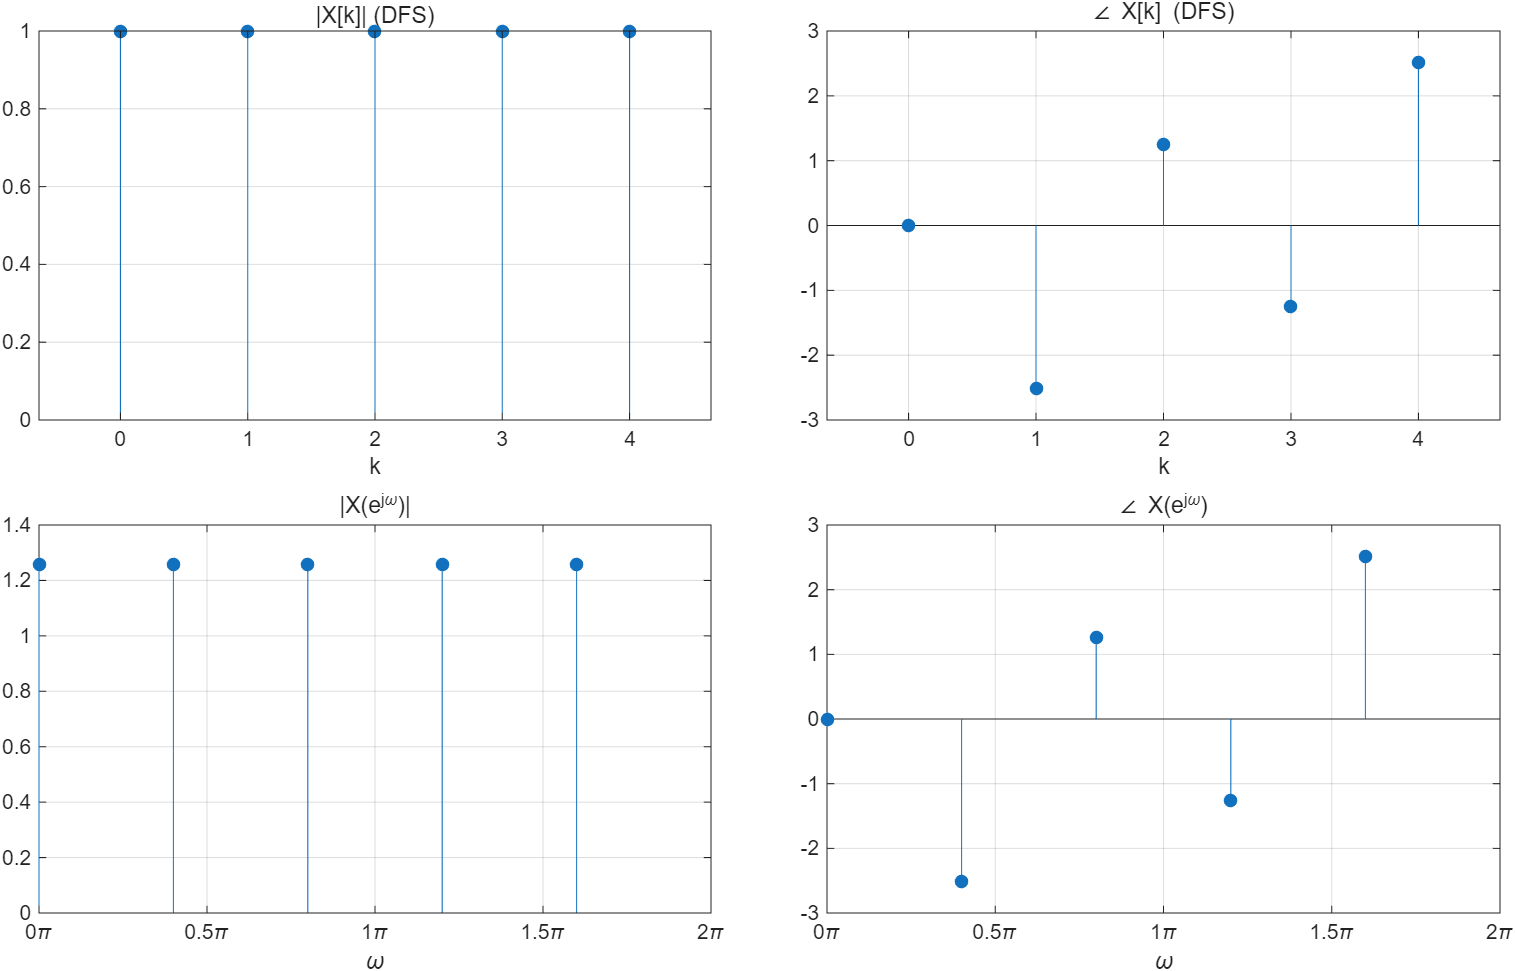
\includegraphics[width=0.8\textwidth]{3-34(b) N=5.png}
    \caption{3-34(b) N=5 DFS与DTFT}
    \label{fig:3-34b}
\end{figure}

3-34(c)的MATLAB仿真图像(DFS的幅度和相位以及DTFT的幅度和相位)见图\ref{fig:3-34c}:

\begin{figure}[htbp]
    \centering
    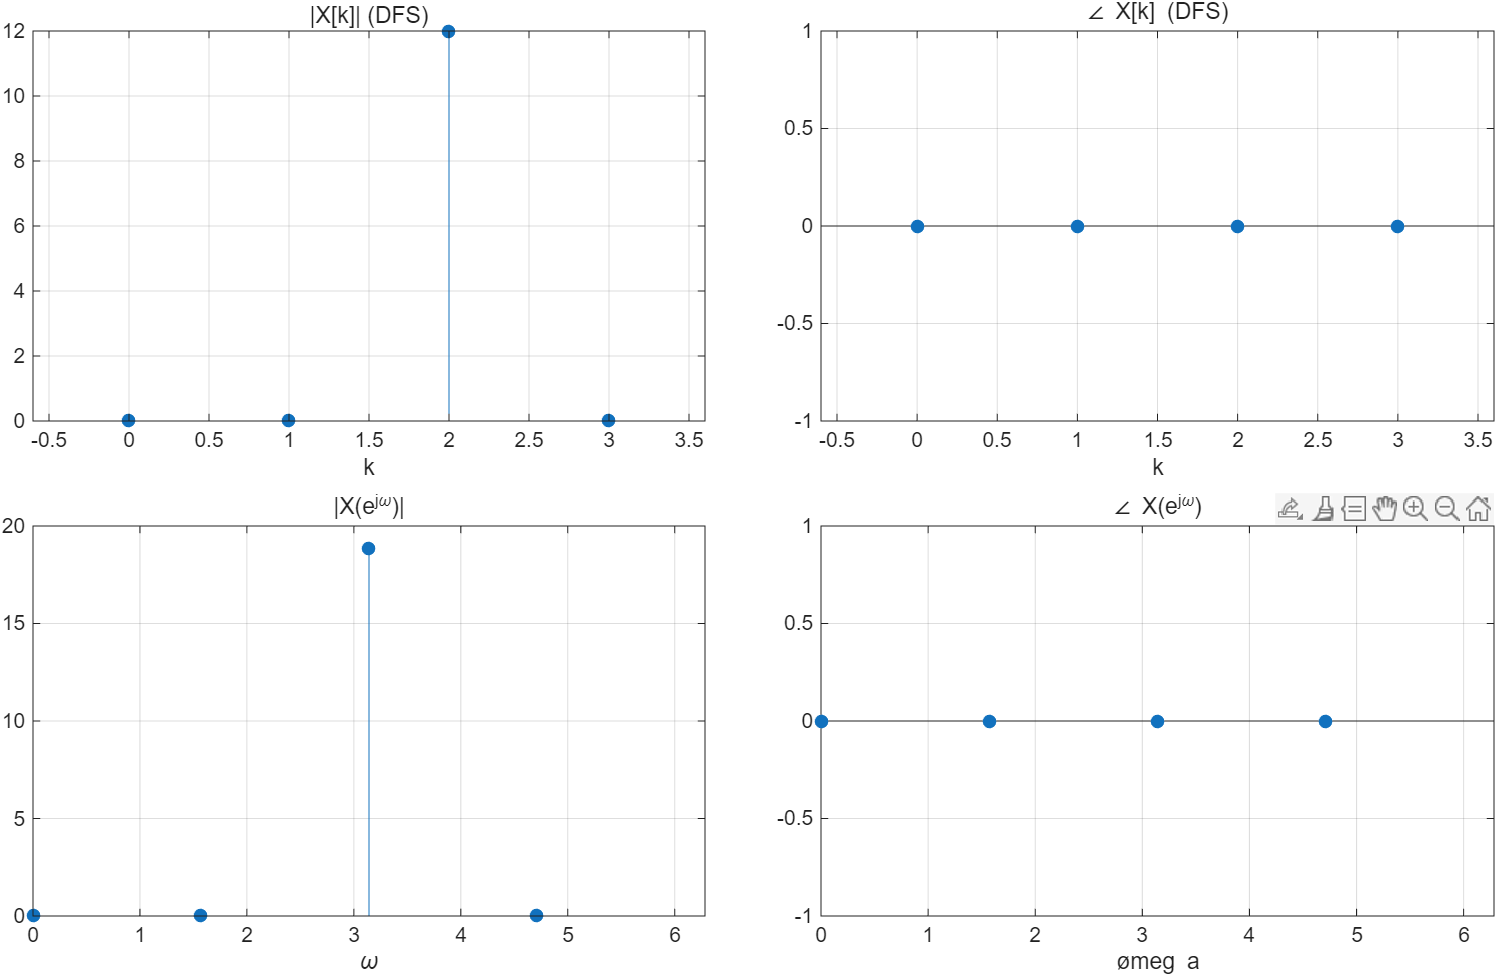
\includegraphics[width=0.8\textwidth]{3-34(c) N=4.png}
    \caption{3-34(c) N=4 DFS与DTFT}
    \label{fig:3-34c}
\end{figure}

\subsection{实验分析}

本节主要分析周期离散时间信号的DFS与DTFT的计算及其关系:

\subsubsection{DFS的理论值}

1. 3-34(a):

$\tilde{x}[n] = \cos(0.8\pi n) + \cos(0.1\pi n)=\frac{1}{2}(e^{j0.8\pi n}+e^{-j0.8\pi n}+e^{j0.1\pi n}+e^{-j0.1\pi n}) = \frac{1}{N}\times 10 (e^{j\frac{2\pi}{N} 8n}+e^{-j\frac{2\pi}{N} 8 n}+e^{j\frac{2\pi}{N}  n}+e^{-j\frac{2\pi}{N} n})$

因此可以发现:
$$\tilde{X}[k]=\sum_{k=-\infty}^{+\infty}\delta[k-8-20k]+\delta[k+8-20k]+\delta[k-1-20k]+\delta[k+1-20k]$$
对应图\ref{fig:3-34a},DFS的幅度在0$\sim$19范围内只在1,8,12,19这四个离散点出现。

2. 3-34(b)
$$\tilde{X}[k]=\sum_{n=0}^{N}\tilde{x}[n]e^{-j\frac{2\pi}{N}kn}=e^{-j0.8\pi k}$$
对应图\ref{fig:3-34b},DFS的幅度在0$\sim$4范围内全为1

3. 3-34(c)
$$\tilde{X}[k]=\sum_{n=0}^{N}\tilde{x}[n]e^{-j\frac{2\pi}{N}kn}=3(1-j^{-k}+(-1)^k-j^k)$$
满足在$k \in [0,3]$范围内,$\tilde{X}[k]$只在$k=3$处取$\tilde{X}[3]=12$,其余点全为0。此外,我们可以发现对于任意$k$,$\tilde{X}[k]$恒为非负实数,因此相位恒为0。符合图\ref{fig:3-34c}中的情况

\subsubsection{周期离散时间信号的DTFT与DFS的关系}

我们假设周期离散时间信号$\tilde{x}[n]$的DFS为: $\tilde{X}[k]$,则其DTFT为:
$$\mathcal{F}\{\tilde{x}[n]\}=\frac{2\pi}{N}\sum_{k=-\infty}^{\infty}\tilde{X}[k]\delta(\omega-k\cdot\frac{2\pi}{N})$$
可见,周期离散时间信号的DTFT相当于是在其DFS频谱上幅度倍乘了$\frac{2\pi}{N}$倍,而相位保持不变,这与3-34的三张图中的情况完全一致。

% ============================================================
% 实验三:4-38 回声系统
% ============================================================
\section{实验三:4-38 回声系统}

\subsection{题目内容}

回声系统的差分方程是 $y[n] = x[n] + 0.5x[n-10]$,画出其零极点图、幅度响应和群延迟。

(提示: 可以调用的函数有 \texttt{zplane()},\texttt{freqz()},\texttt{grpdelay()} 等)

\subsection{实验结果}

实验结果见图\ref{fig:4-38}:

\begin{figure}[htbp]
    \centering
    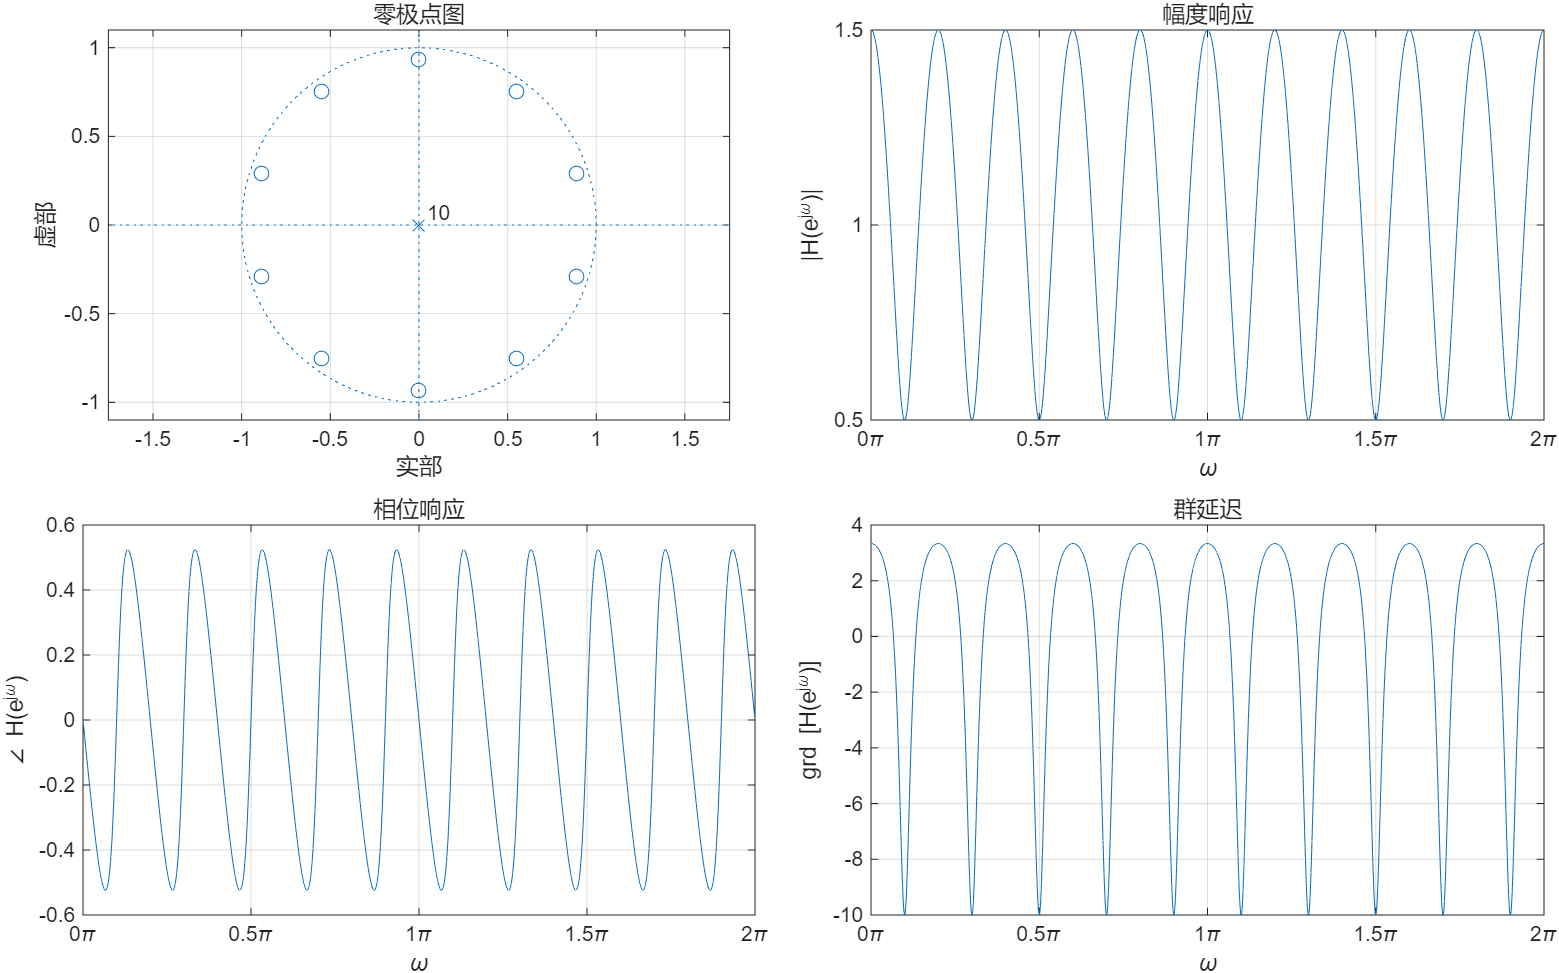
\includegraphics[width=0.8\textwidth]{4-38 回声系统.png}
    \caption{4-38 回声系统的零极点图、幅度响应、相位响应和群延迟}
    \label{fig:4-38}
\end{figure}

\subsection{实验分析}

原系统的系统函数:
$$H(z)=1+\frac{1}{2}z^{-10}$$
令$H(z)=0: z^{10}=-\frac{1}{2}$

解的:
$$z_k=(\frac{1}{2})^{1/10}e^{j(\pi + k\cdot 2\pi)/N}, k=0,1,2,...,9$$
因此零点必然环绕在圆: $r=(\frac{1}{2})^{1/10}$附近,这与图\ref{fig:4-38}中的零极点图相同。

频率响应为:$$H(e^{j\omega})=1+\frac{1}{2}e^{-j10\omega}$$
幅度响应:$$|H(e^{j\omega})|=\sqrt{(1+\frac{1}{2}\cos{10\omega})^2+\frac{1}{4}\sin^2{10\omega}}$$
相位响应:$$\angle [H(e^{j\omega})] = \arctan \frac{-1/2\sin{10\omega}}{1+1/2\cos{10\omega}}$$

% ============================================================
% 实验四:4-39 滑动平均系统与其延迟互补系统
% ============================================================
\section{实验四:4-39 滑动平均系统与其延迟互补系统}

\subsection{题目内容}

已知滑动平均系统的单位脉冲响应是 $h_M[n] = \frac{1}{M}R_M[n]$,其延迟互补系统的单位脉冲响应是
$$
g_M[n] = \frac{\sin\left[\pi\left(n - \frac{M-1}{2}\right)\right]}{\pi\left(n - \frac{M-1}{2}\right)} - h_M[n]
$$
分别画出当 $M=2$、$3$、$4$ 和 $5$ 时两个系统的零极点图、幅度响应和相位响应。分别是哪类广义线性相位 FIR 系统?

(提示: 可以调用的函数有 \texttt{zplane()} 和 \texttt{freqz()} 等)

\subsection{实验结果}

MATLAB计算得到序列$h_{M}[n]$和$g_{M}[n]$的值分别是:

\begin{verbatim}
--------------------------------------
M=2
hm序列:
    0.5000    0.5000

gm序列:
    0.1366    0.1366

--------------------------------------
M=3
hm序列:
    0.3333    0.3333    0.3333

gm序列:
   -0.3333    0.6667   -0.3333

--------------------------------------
M=4
hm序列:
    0.2500    0.2500    0.2500    0.2500

gm序列:
   -0.4622    0.3866    0.3866   -0.4622

--------------------------------------
M=5
hm序列:
    0.2000    0.2000    0.2000    0.2000    0.2000

gm序列:
   -0.2000   -0.2000    0.8000   -0.2000   -0.2000
\end{verbatim}

$M=2$时,两个系统的零极点图、幅度响应和相位响应见图\ref{fig:4-39-m2}:

\begin{figure}[htbp]
    \centering
    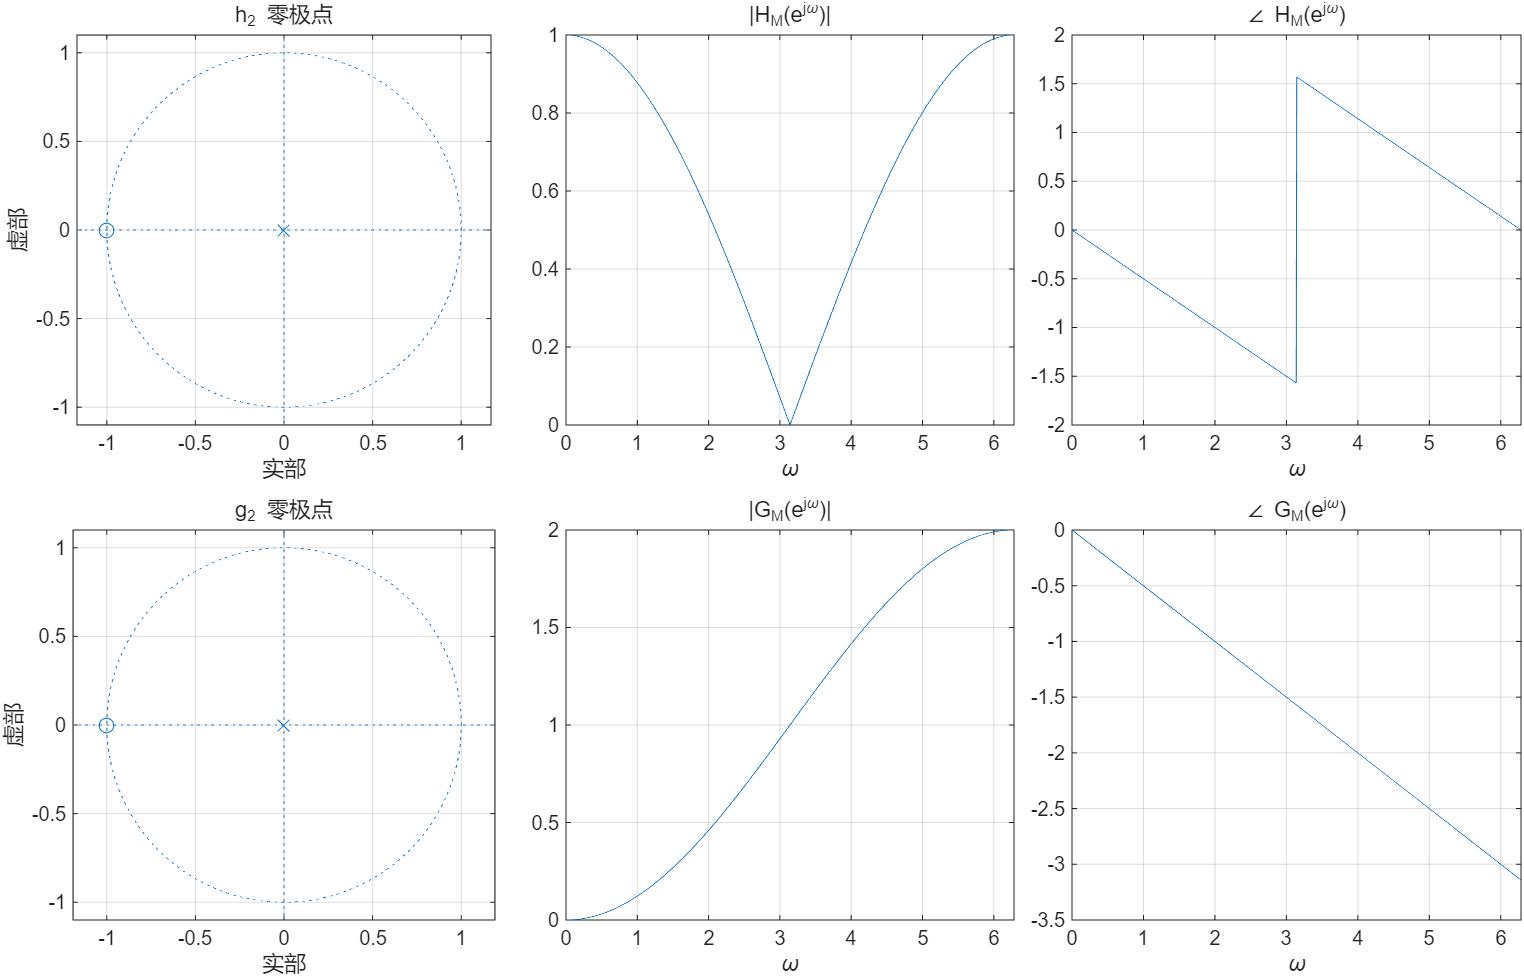
\includegraphics[width=0.9\textwidth]{4-39_M=2.png}
    \caption{4-39 M=2 滑动平均系统与延迟互补系统}
    \label{fig:4-39-m2}
\end{figure}

$M=3$时,两个系统的零极点图、幅度响应和相位响应见图\ref{fig:4-39-m3}:

\begin{figure}[htbp]
    \centering
    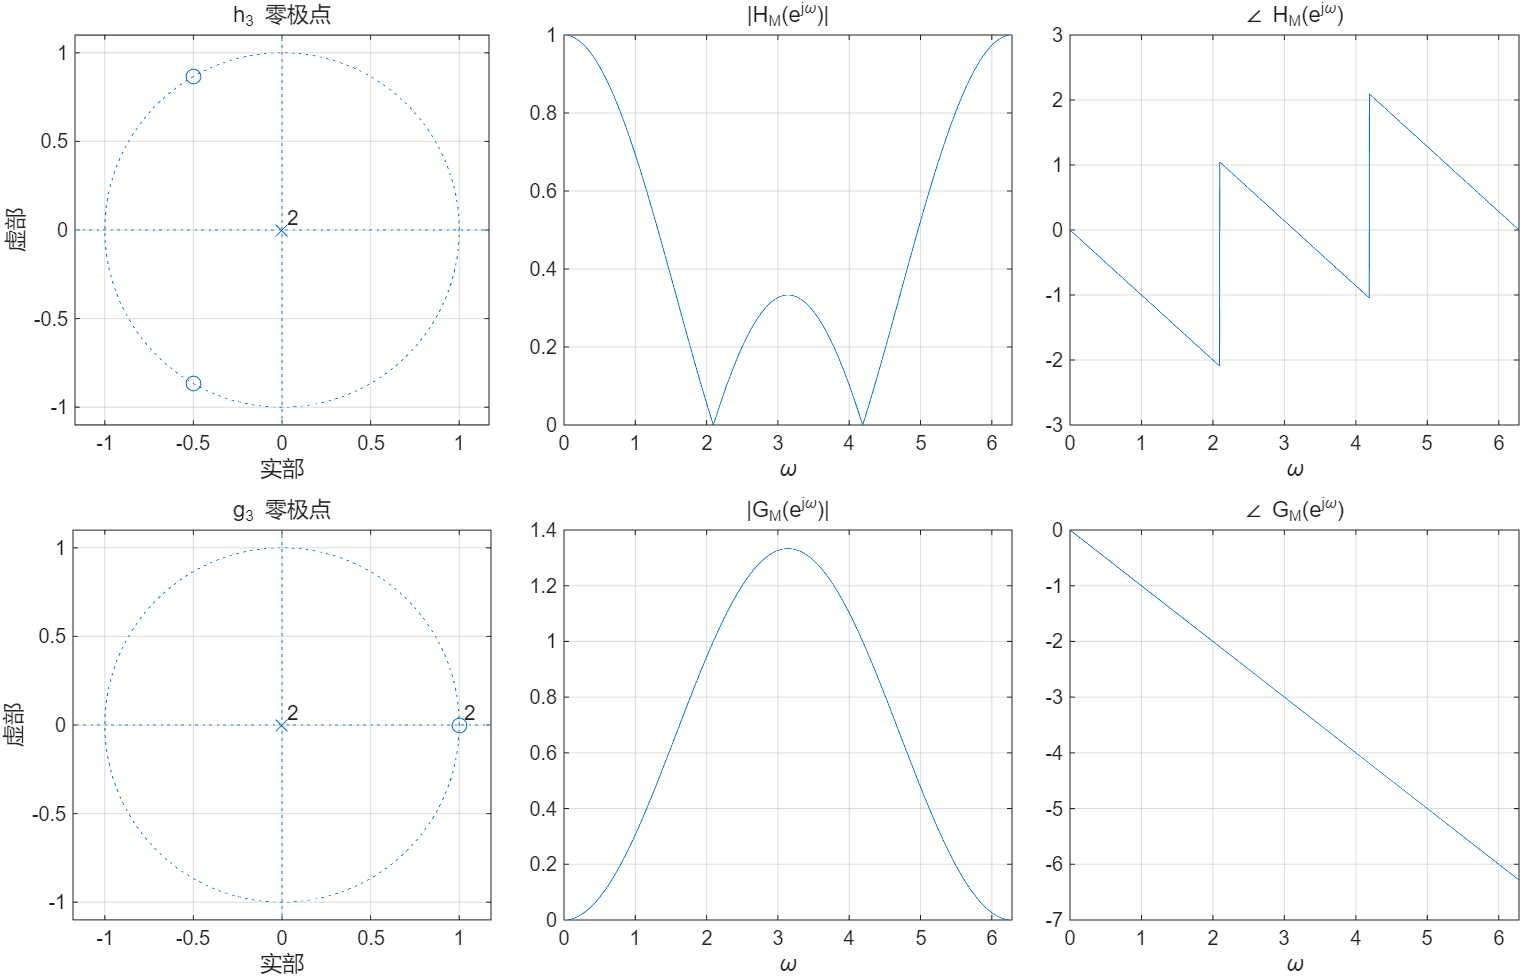
\includegraphics[width=0.9\textwidth]{4-39_M=3.png}
    \caption{4-39 M=3 滑动平均系统与延迟互补系统}
    \label{fig:4-39-m3}
\end{figure}

$M=4$时,两个系统的零极点图、幅度响应和相位响应见图\ref{fig:4-39-m4}:

\begin{figure}[htbp]
    \centering
    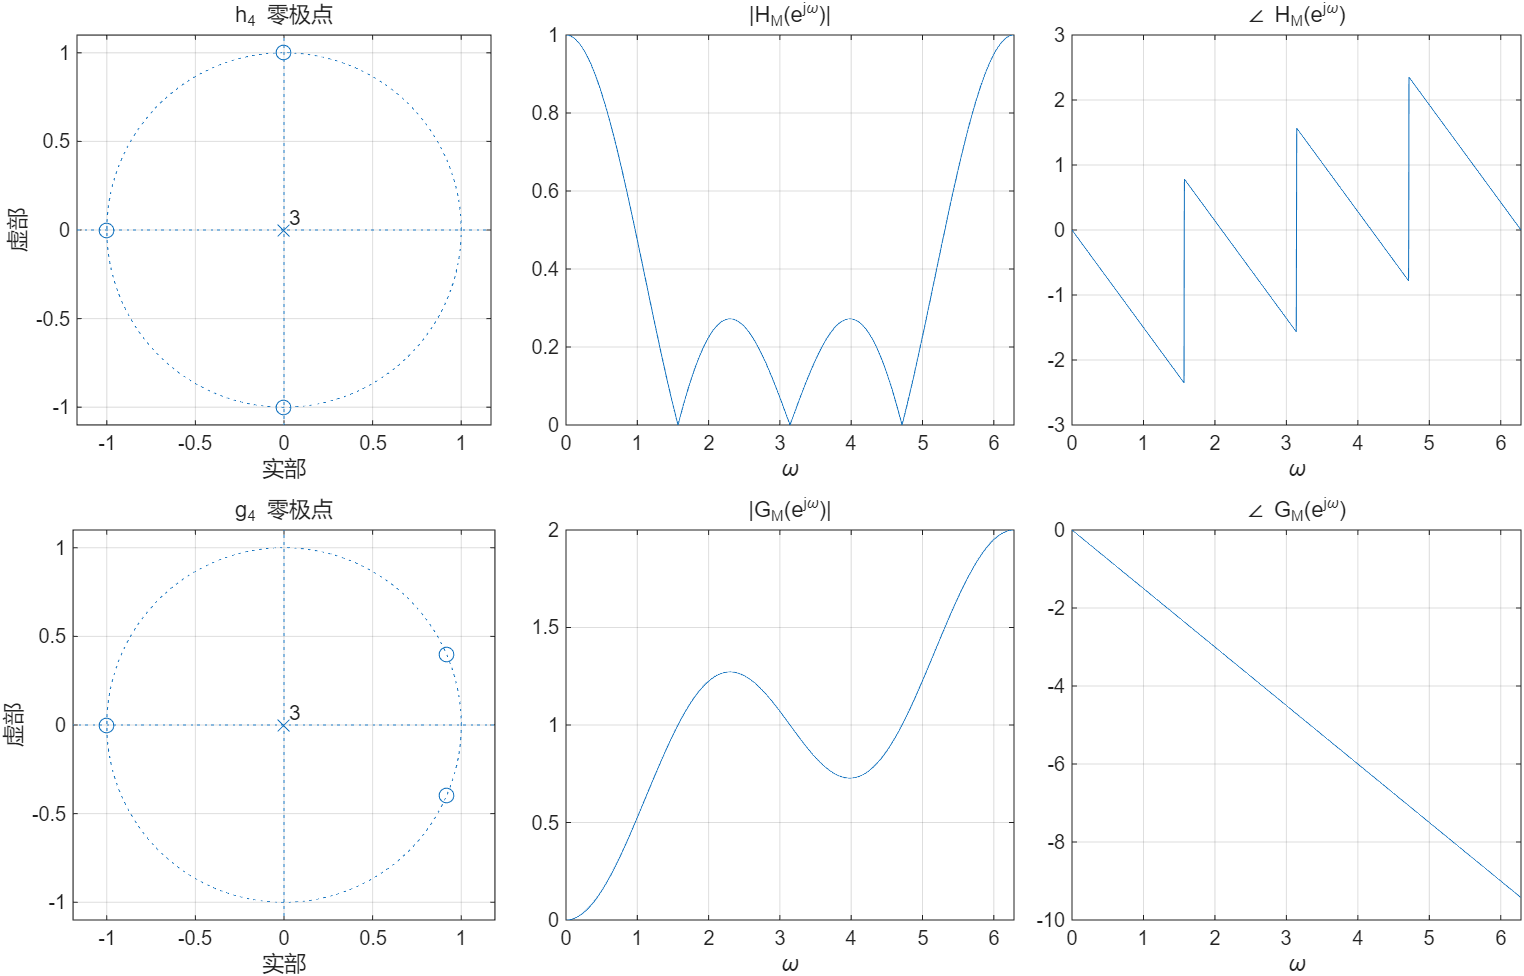
\includegraphics[width=0.9\textwidth]{4-39_M=4.png}
    \caption{4-39 M=4 滑动平均系统与延迟互补系统}
    \label{fig:4-39-m4}
\end{figure}

$M=5$时,两个系统的零极点图、幅度响应和相位响应见图\ref{fig:4-39-m5}:

\begin{figure}[htbp]
    \centering
    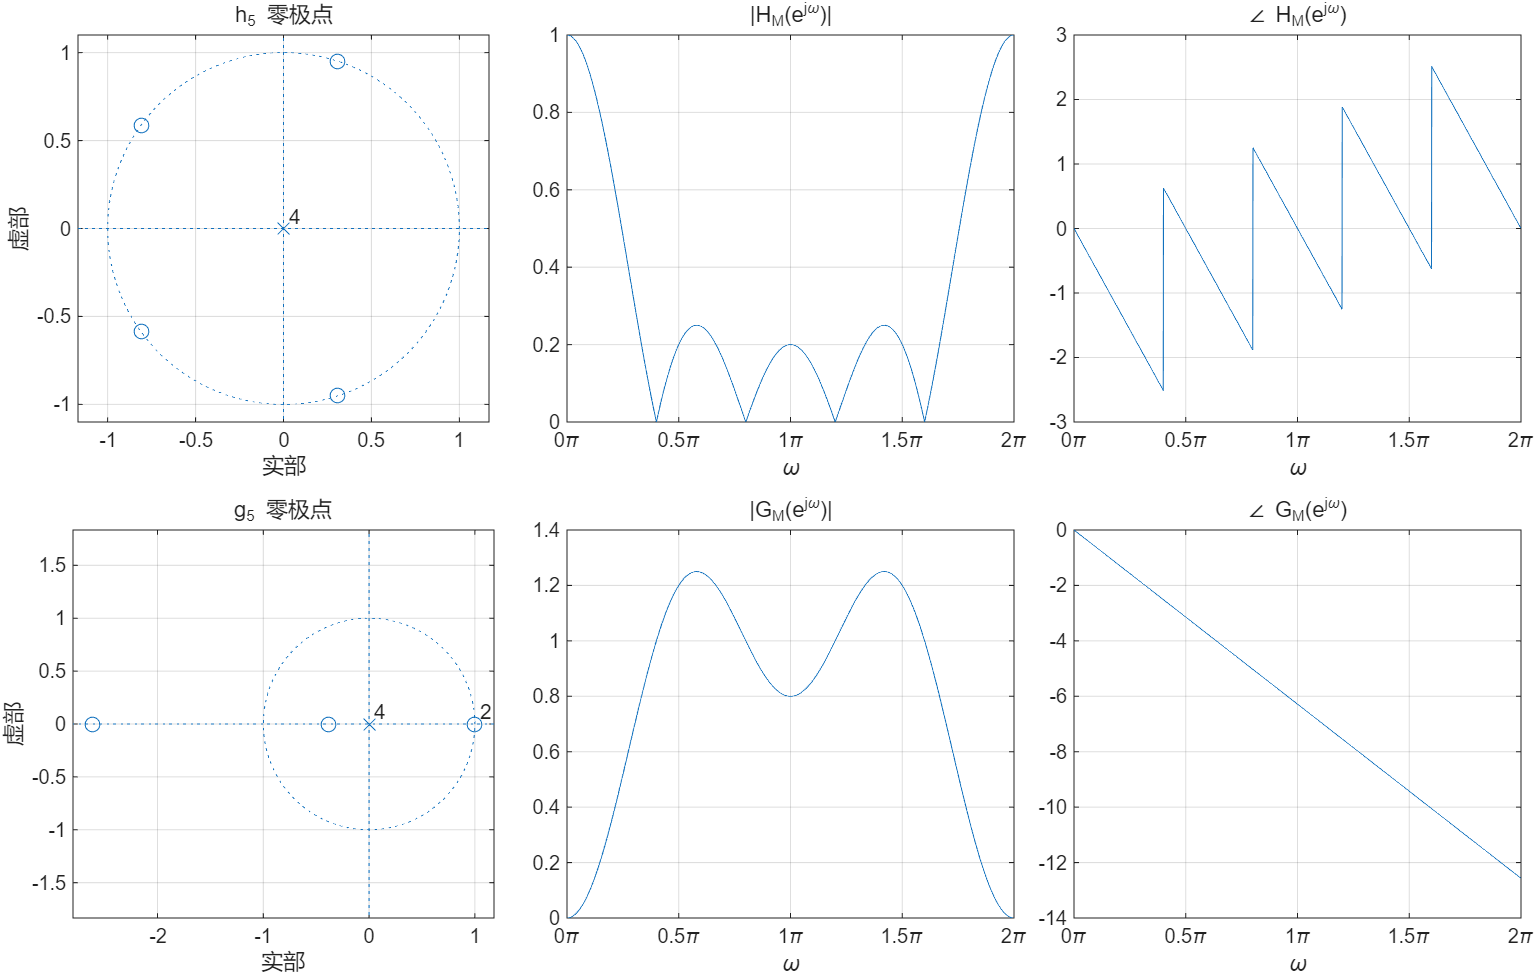
\includegraphics[width=0.9\textwidth]{4-39_M=5.png}
    \caption{4-39 M=5 滑动平均系统与延迟互补系统}
    \label{fig:4-39-m5}
\end{figure}

\subsection{实验分析}

已知对于任意: $M \geq 1$,序列: $\text{sinc}[\pi(n - \frac{M-1}{2})]$和$h_{M}[n]$均关于$n=\frac{M-1}{2}$偶对称,因此序列$g_{M}[n]$也关于$n=\frac{M-1}{2}$偶对称。并且:

1. 当 $M$ 为偶数,即$M=2,4$时,满足$x[n] = x[M-1-n]$,$M-1$是奇数,因此两个系统都是II类系统

2. 当 $M$ 为奇数,即$M=3,5$时,满足$x[n] = x[M-1-n]$,$M-1$是偶数,因此两个系统都是I类系统

这几个序列也都是实序列,因此幅度响应关于$\omega = k\pi$偶对称,相位响应关于$\omega = k\pi$奇对称

频率响应:
$$X(e^{j\omega})=e^{-j\omega\frac{M}{2}}\sum_{n=0}^{M}x[n]\cos[\omega(n-\frac{M}{2})]$$
其中相位响应为:

$$
\angle [X(e^{j\omega})] = \left\{
\begin{aligned}
& -\frac{M}{2}\omega & \sum_{n=0}^{M}x[n]\cos[\omega(n-\frac{M}{2})] > 0 \\
&  -\frac{M}{2}\omega + \pi & \sum_{n=0}^{M}x[n]\cos[\omega(n-\frac{M}{2})] < 0\\
\end{aligned}
\right.
$$

即相位响应是$\omega$的分段线性函数,这一点在4-39的图中也能得到体现

此外,我们知道,$M=2, 4$时$h_M[n]$和$g_M[n]$都是II类系统,观察它们的零极点图可以发现,它们均在$z=-1$处有一个零点,符合对称系统的零点特性。

% ============================================================
% 附录:MATLAB代码
% ============================================================
\newpage
\section{附录:MATLAB代码}

\subsection{实验一代码:3-31}

\begin{lstlisting}
%% 3-31 有限长序列的 DTFT 幅度与相位
%% 采用freqz(b, a, w)函数的方法求解DTFT
%% b分子系数,a分母系数,w采样的频率点个数
clear; clc; close all;
seqs = {
    [4 3 2 1 2 3 4],              '3-31(a)';
    [4 3 2 1 0 -1 -2 -3 -4],      '3-31(b)';
};

for i = 1:size(seqs,1)
    x = seqs{i,1}; 
    label = seqs{i,2};
    [X, w] = freqz(x, 1, 4096, 'whole');   % 用 freqz 计算"以 x 为 FIR 系数(分子),分母为 1"的频响。

    figure('Name', label, 'NumberTitle','off');                         % 新建图窗,名称用 label,且不显示默认编号。
    t = tiledlayout(2,1, 'Padding','compact','TileSpacing','compact');  % 创建 2 行 1 列的网格布局,压缩边距与间距,便于紧凑显示两幅图。
    % figure 1
    nexttile; 
    plot(w, abs(X)); 
    grid on; 
    xlim([0 2*pi]);
    xticks(0:0.5*pi:2*pi);
    xticklabels(string(0:0.5:2) + "\pi");
    xlabel('\omega'); 
    ylabel('|X(e^{j\omega})|');
    title([label ' 幅度']);

    % figure 2
    nexttile; 
    plot(w, unwrap(angle(X)));   % unwrap 去除 2π 跳变,使相位连续
    grid on; 
    xlim([0 2*pi]);
    xticks(0:0.5*pi:2*pi);
    xticklabels(string(0:0.5:2) + "\pi");
    xlabel('\omega'); 
    ylabel('\angle X(e^{j\omega})'); 
    title([label ' 相位']);
end
\end{lstlisting}

\subsection{实验二代码:3-34}

\begin{lstlisting}
%% 3-34 周期序列的 DFS 与 DTFT
% 周期序列在一个周期内的 DFT 就是该周期序列的 DFS
% 周期序列的 DTFT 为在 ω_k=2πk/N 处的"冲激",权重 2π X[k]。
% 与非周期离散时间信号的DTFT谱不同,周期离散时间信号的谱是冲激谱,需要用stem作图
clear; clc; close all;
cases = {
    20, @(n) cos(0.8*pi*n) + cos(0.1*pi*n), '3-34(a) N=20';
    5,  @(n) [0 0 1 0 0],                   '3-34(b) N=5';
    4,  @(n) [3 -3 3 -3],                   '3-34(c) N=4';
};

for i = 1:size(cases,1)
    N = cases{i,1};   % 周期
    f = cases{i,2};   % 序列
    name = cases{i,3}; % 序列名称
    n = 0:N-1; 
    x = f(n);            % 取出一段周期样本
    x = x(1:N);          % 一段周期样本
    Xk = fft(x);         % FFT(x)计算出一段周期样本信号的DFT系数,等效为该周期信号的傅里叶级数系数
    wk = 2*pi*(0:N-1)/N;

    figure('Name', name, 'NumberTitle','off');
    % DFS幅度
    t = tiledlayout(2,2, 'Padding','compact','TileSpacing','compact');
    nexttile; 
    stem(0:N-1, abs(Xk), 'filled'); 
    grid on;
    xlabel('k'); 
    title('|X[k]| (DFS)');

    % DFS 相位
    nexttile; 
    stem(0:N-1, angle(Xk), 'filled'); 
    grid on;
    xlabel('k'); 
    title('\angle X[k] (DFS)');

    % DTFT 幅度
    nexttile; 
    stem(wk, 2*pi/N*abs(Xk), 'filled'); 
    grid on; 
    xlim([0 2*pi]);
    xticks(0:0.5*pi:2*pi);
    xticklabels(string(0:0.5:2) + "\pi");
    xlabel('\omega'); 
    title('|X(e^{j\omega})|');

    % DTFT 相位
    nexttile; 
    stem(wk, angle(Xk), 'filled'); 
    grid on; 
    xlim([0 2*pi]);
    xticks(0:0.5*pi:2*pi);
    xticklabels(string(0:0.5:2) + "\pi");
    xlabel('\omega'); 
    title('\angle X(e^{j\omega})');
end
\end{lstlisting}

\subsection{实验三代码:4-38}

\begin{lstlisting}
%% 4-38 回声系统 y[n] = x[n] + 0.5 x[n-10]
clear; clc; close all;

b = [1, zeros(1,9), 0.5];  % 分子系数
a = 1;   % 分母系数

[H, w] = freqz(b, a, 2048, 'whole');      % freqz求解频率响应
[gd, wg] = grpdelay(b, a, 2048, 'whole'); % grpdelay求解群延迟

figure('Name','4-38 回声系统', 'NumberTitle','off');
t = tiledlayout(2,2, 'Padding','compact','TileSpacing','compact');

% 零极点图
nexttile; 
zplane(b,a);   % zplane函数求解零极点图
grid on; 
title('零极点图');

% 幅度响应
nexttile; 
plot(w, abs(H)); 
grid on; 
xlim([0 2*pi]);
xticks(0:0.5*pi:2*pi);
xticklabels(string(0:0.5:2) + "\pi");
xlabel('\omega'); 
ylabel('|H(e^{j\omega})|')
title('幅度响应');

% 相位响应
nexttile; 
plot(w, unwrap(angle(H))); 
grid on; 
xlim([0 2*pi]);
xticks(0:0.5*pi:2*pi);
xticklabels(string(0:0.5:2) + "\pi");
xlabel('\omega'); 
ylabel('\angle H(e^{j\omega})')
title('相位响应');

% 群延迟
nexttile; 
plot(wg, gd); 
grid on; 
xlim([0 2*pi]);
xticks(0:0.5*pi:2*pi);
xticklabels(string(0:0.5:2) + "\pi");
xlabel('\omega'); 
ylabel('grd [H(e^{j\omega})]'); 
title('群延迟');
\end{lstlisting}

\subsection{实验四代码:4-39}

\begin{lstlisting}
%% 4-39 滑动平均系统与其延迟互补系统
% h_M[n] = (1/M) * rect_M[n]
% g_M[n] = sinc(n-(M-1)/2) - h_M[n]
clear; clc; close all;

Mlist = 2:5;

for M = Mlist
    disp("--------------------------------------");
    fprintf("M=%d\n", M);
    b = ones(1, M) / M;     % 滑动平均 FIR 系数
    seq = 0 : (M-1);
    b_g = sinc(seq - (M-1)/2) - b;
    disp("hm序列:");
    disp(b);
    disp("gm序列:");
    disp(b_g);
    a = 1;

    % 滑动平均系统
    [H, w] = freqz(b, a, 2048, 'whole');   % 0..2π

    % 延迟互补系统
    [G, ww] = freqz(b_g, a, 2048, 'whole');

    figure('Name', sprintf('4-39_M=%d', M), 'NumberTitle','off');
    t = tiledlayout(2,3, 'Padding','compact','TileSpacing','compact');

    % h_M 零极点
    nexttile; 
    zplane(b, a); 
    grid on; 
    title(sprintf('h_{%d} 零极点',M));

    % h_M 幅度
    nexttile; 
    plot(w, abs(H)); 
    grid on; 
    xlim([0 2*pi]);
    xticks(0:0.5*pi:2*pi);
    xticklabels(string(0:0.5:2) + "\pi");
    xlabel('\omega');  
    title('|H_M(e^{j\omega})|');

    % h_M 相位
    nexttile; 
    plot(w, unwrap(angle(H))); 
    grid on; 
    xlim([0 2*pi]);
    xticks(0:0.5*pi:2*pi);
    xticklabels(string(0:0.5:2) + "\pi");
    xlabel('\omega'); 
    title('\angle H_M(e^{j\omega})');

    % g_M 零极点图
    nexttile; 
    zplane(b_g, a); 
    grid on; 
    title(sprintf('g_{%d} 零极点',M));

    % g_M 幅度
    nexttile; 
    plot(w, abs(G)); 
    grid on; 
    xlim([0 2*pi]);
    xticks(0:0.5*pi:2*pi);
    xticklabels(string(0:0.5:2) + "\pi");
    xlabel('\omega'); 
    title('|G_M(e^{j\omega})|');

    % g_M 相位
    nexttile; 
    plot(w, unwrap(angle(G))); 
    grid on; 
    xlim([0 2*pi]);
    xticks(0:0.5*pi:2*pi);
    xticklabels(string(0:0.5:2) + "\pi");
    xlabel('\omega'); 
    title('\angle G_M(e^{j\omega})');

end

%% 工具函数:归一化 sinc
function y = sincn(x)
% sin(pi x)/(pi x),x=0 处定义为 1
y = ones(size(x));
idx = abs(x) > eps;   % 如果x=0,保持该点的初值:1
y(idx) = sin(pi*x(idx))./(pi*x(idx));
end
\end{lstlisting}







\end{document}
